\documentclass[a4paper,12pt]{article}
\usepackage{blindtext}
\usepackage[utf8]{inputenc}
\usepackage{hyperref}
\usepackage{graphicx}

\begin{document}

\begin{titlepage}

\newcommand{\HRule}{\rule{\linewidth}{0.5mm}} % Defines a new command for the horizontal lines, change thickness here

\center % Center everything on the page
 
%----------------------------------------------------------------------------------------
%	HEADING SECTIONS
%----------------------------------------------------------------------------------------

\textsc{\LARGE University of Pretoria}\\[1.5cm]
\textsc{\Large COS 301 - Software Engineering}\\[0.5cm]
\textsc{\large Team Fox}\\[0.5cm]

%----------------------------------------------------------------------------------------
%	TITLE SECTION
%----------------------------------------------------------------------------------------

\HRule \\[0.4cm]
{ \huge \bfseries Software Requirements Specification and Technology Neutral Process Design}\\[0.4cm] % Title of your document
\HRule \\[1.5cm]
 
%----------------------------------------------------------------------------------------
%	AUTHOR SECTION
%----------------------------------------------------------------------------------------

\begin{minipage}{0.4\textwidth}
\begin{flushleft} \large
\emph{Author(s):}\\
Gian Paolo \textsc{Buffo} % Your name
\end{flushleft}
\end{minipage}
~
\begin{minipage}{0.4\textwidth}
\begin{flushright} \large
\emph{Student number(s):} \\
14446619 % Student number
\end{flushright}
\end{minipage}\\[4cm]


%----------------------------------------------------------------------------------------
%	DATE SECTION
%----------------------------------------------------------------------------------------

{\large \today}\\[3cm] % Date, change the \today to a set date if you want to be precise

 
%----------------------------------------------------------------------------------------

\vfill % Fill the rest of the page with whitespace

\end{titlepage}

\newpage

%=========================================READ ME========================================
%----------------------------------------------------------------------------------------
% I have randomly assigned questions to all of us to get the ball rolling. Obviously,
% anyone can contribute to anything if they feel they have something to add/change.
% The names will be above each section.
% - GP
%----------------------------------------------------------------------------------------


%----------------------------------------------------------------------------------------
% Done by: Jason Gordon (edited by Gian Paolo Buffo)
%----------------------------------------------------------------------------------------
\section{Introduction}

The requirements specification should ultimately contain sufficient information such that the system could be largely developed by a third party without further input. To this end the requirements must be precise and testable.

The requirements need not be fully specified up-front. One might start with the vision, scope and architectural requirements, perform an upfront software architecture engineering phase and then iteratively elicit the detailed requirements for a use case; build, test and deploy the use case before adding the detailed requirements for the next use case.

Such an approach follows solid engineering practices for the core software infrastructure architecture with an agile software development approach within which the application functionality is developed iteratively.

%----------------------------------------------------------------------------------------
% Done by: Gian Paolo Buffo
%----------------------------------------------------------------------------------------
\section{Vision}

With the implementation of this system, the client is trying to create a central piece of software that can be used by all staff members of the Computer Science department of the University of Pretoria to maintain their academic publications.

However, the software will provide much greater functionality than merely listing all publications. One of the main features of the system will be the ability to add and edit publications, as well as specify a multitude of metadata items such as the title, (co)-authors, deadlines, progress towards completion, status (published, accepted, submitted etc.) and intended venue (conference, journal).

Additionally, the system will be used to provide users (who are authors of publications) with all manner of information regarding their Research Output Units and funding. This includes information such as expected units and funding, obtained units and funding, and shortfall of units.

The system will provide outputs in the form of an Excel spreadsheet which will illustrate the aforementioned author details both in a tabular fashion and graphically, most likely in the form of bar and/or line graphs. A sheet will be generated for each individual author, and a master sheet will be generated for the Research Leaders and Head of Department respectively.

A typical usage scenario of the system will be as follows:
\begin{itemize}

\item A user, who in this case is an author as well as the Head of Department (giving him/her administrator rights), logs in to the system.
\item The user then adds a new publication on his/her profile page, filling in the relevant metadata items. The user will by default be added as an author.
\item The user realises that he/she made an error while filling in the title, and edits the title appropriately.
\item The units corresponding to the publication's venue (which have been assigned by the system) are automatically added to the user, and all unit-related calculations are made
\item The user's profile page is updated with the new publication and all related information.
\item The user then chooses to generate the Excel document which contains not only information about his/her Research Output Units and funding in a tabular and graphical fashion, but also similar information for all other members of the department, who are users. This is because the user has Head of Department rights. 

\end{itemize}

%----------------------------------------------------------------------------------------
% Done by: Jacques van Wyk (edited by Gian Paolo Buffo)
%----------------------------------------------------------------------------------------
\section{Background}

Our group, Team Fox, had a meeting with the client, Ms Vreda Pieterse, on Wednesday, 17 February 2016. The client discussed that she requires the implementation of a system which will allow researchers to keep track of their publications, as well as view statistical information regarding their Research Output Units.

We have been given this topic for our mini project for the module COS 301. Furthermore, the mini project is to train us and help assist us in readying ourselves for the main project of this module.

This will give our group, Team Fox, the opportunity to gain experience on how to put together an SRS (Software Requirements Specification) that will help us and the client to better understand what is needed from the system and its functionality and how they would like to interact with the system. Consequently, if we better understand what our client wants the system to be, it will give us a better opportunity to implement a system that the client will be pleased with and which the client will want to use.
 	
In addition, the system will be used by the Computer Science department at the University of Pretoria. Hopefully the system will improve on the system(s) currently in use and will provide a basic structure of good quality which will enable it to be updated and improved in the future of its software development life cycle.
 	
Furthermore, the project might serve as an example to other students on how to implement such a system or it can be used as a basic structure and starting point for other institutes.

\section{Architecture Requirements}

The software architecture requirements include the access and integration requirements, quality
requirements and architectural constraints.

%----------------------------------------------------------------------------------------
% Done by: Hlengekile Jita (edited by Gian Paolo Buffo)
%----------------------------------------------------------------------------------------
\subsection{Access Channel Requirements}

When considering the access channels of a target system, there are two main possibilities to consider: the human users of the system and whether any other systems need to be able to access the system. For both of these possibilities one then needs to consider through which ways they will access the system, what functionality the system requires these access channels to have and how these access channels will provide said functionality. 

The system required by our client (which will from herewith be referred to as the system or the target system) is a system through which researchers can keep track of their publications. The users of the system, the researchers, need a channel through which they can use the system. The client does not require any other systems to be able to access our system or use the functionality of our system for a higher processing scheme, at this stage.

The client would like the creation of two platforms through which the users of the system can access the system, namely:
\begin{itemize}
	\item A Web Interface
	\item A Mobile Application (On the Android platform)
\end{itemize}

Both of these will have to access our system through the Internet - for the Android Application, this will require requesting permissions. The aforementioned platforms will need an interface through which to access our system, known as an Application Programming Interface (API). This interface will have to enable the passing of data from the system to the channel through which the user accesses the system. Considering the general functionality our system provides, and that communication would take place through the Internet, this API would have to be RESTful.

REST stands for Representational State Transfer, and it is a software architectural style that deals with resources and what resources are accessed through using the HTTP user-oriented network protocol. This RESTful API would enable the transfer of data between our system and the platforms our client has chosen for users to access the system through - in our case over a network, namely the Internet.

Before we consider this API further and what data it shall pass and how our access channels will use the API, let us revisit the functionality the access platforms will need to have to provide the users with the target system's maximum functionality.
\begin{itemize}
	\item User log in
	\item Search functionality
	\item Ability to open excel spreadsheets
	\item Viewing of plain text
	\item Viewing of lists, tables etc.
	\item Viewing of links
	\item Ability to view information
	\item Ability to add information
	\item Ability to change information
	\item Ability to remove information
\end{itemize}

For the viewing of text, lists, links and the like, this will have to do with the Graphical User Interface (GUI) that the access channel provides. In the case of the Web Interface this can be designed using HTML and its associated counterparts such as CSS, Bootstrap and more. In the case of the Android Application, a number of classes and functions will be used. For example in the case of a list, one would use a ListView item on their user interface and this can be created using the android.widget.ListView class, and operations on said list will be done using the classes' associated functions.

The Search functionality would also need to be provided by the Graphical User Interface, but actual searching of the database used in our system will be done by the system itself, so our API would need to be able to request the system to do the search, when a user provides the required information for the search by interacting with the GUI.

For the ability to open Excel spreadsheets, in the Web Interface, this would imply the ability to download a file; while on an Android Application, this would imply the same thing as well as the improved ability to open the user devices' spreadsheet viewer.

As for the user log in functionality, users would provide user details through the GUI and the API would then need to pass user details for verification to the system and be able to receive a response about whether or not log in was successful or not. Another option that would be safer is the use of API authentication, this is a token based authentication in which the user would log in and if successful the system will respond with a unique token that can be used in future requests.

As we already know the information that will be displayed on these platforms GUIs will be provided through the RESTful API from our system. For this information, the API would need to get information from the system and be able to send changes including the addition and removal of information back to the system. Basically all the interaction between the system and these platforms will be done by the API with the following HTTP methods:
\begin{itemize}
	\item GET – For reading information from the system
	\item PUT – For adding information to the system
	\item DELETE – For removing information from the system
	\item POST – For making changes/edits to information on the system
	\item OPTIONS – For getting operations that can be performed by the system
\end{itemize}

While these platforms vary, they will both access the system through this API and use the Internet to communicate with the system. However the ways they call the API, process and deal with the responses will vary slightly on the two platforms. The API would provide a standard way for accessing the system despite what channel may be in use. These access channels thus simply need to provide users with the functionality that the target system requires on a GUI and use the API for providing users with the results and information from the system.
\\\\
\textbf{References}
\begin{itemize}
\item \url{http://www.andrewhavens.com/posts/20/beginners-guide-to-creating-a-rest-api/}
\item \url{http://www.tutorialspoint.com/restful/restful_introduction.htm}
\end{itemize}

%----------------------------------------------------------------------------------------
% Done by: Josef Alberts (edited by Gian Paolo Buffo)
%----------------------------------------------------------------------------------------
\subsection{Quality Requirements}

\subsubsection{Performance}
The system must work as efficiently as possible and not lag in delivering information to the user. Since this system will not be sending large amounts of data, it should not be difficult for the system to transfer the data speedily. In this implementation, we expect the network speed to dictate performance – not the system itself. Regardless, the system must be able to handle the full amount of users (approx. 100) concurrently without experiencing significant delays or errors. The success of this requirement can be measured in the time taken for a task to be completed under normal, and heavy-load scenarios

\subsubsection{Reliability}
It is imperative that the system not experience unnecessary downtime (period of in-operation of the system), thus preventing users from checking on or altering information on the system. An optimal uptime (period of normal operation of the system) within a month would be 99\% and upwards. Additionally there should not be frequent errors within normal operating parameters of the system. This means that simple logins (sessions), alterations or additions to the database should not cause errors which affect the system as a whole. Additionally, minor human errors, such as omission of information, should not be allowed to propagate through the system. But the system should rather allow the user to fix the error immediately – which will also contribute towards the accuracy of information in the database.

\subsubsection{Scalability}
The system will initially be implemented to manage papers pertaining to one faculty, but it might be necessary in the future to expand it to manage more faculties. The maximum amount for one implementation to manage should not exceed 11, and as such it should be scalable to that amount of faculties and the users associated with them. We make the assumption that the total users per faculty does not exceed 100 and, thus, the total on the system will never exceed 1100.

\subsubsection{Usability} 
Users must be able to login, edit information and logout without hassle. The interface should not be cluttered and should not contain redundant information. As management of information on the system is critical, accessing said information should be as simple as possible.

\subsubsection{Auditability}
In order to track changes and/or errors on the system, all actions by users must be logged as they occur. This includes, but is not limited to, log-in attempts, editing of information (whether successful or not) and log-outs. All errors should also be logged in order to simplify error-tracking. The logging system must not interfere with the users' actions and must not significantly affect performance. Logs must be timestamped and must contain information on which user executed an action – or where an error occurred.

\subsubsection{Security}
The system will be protected by a login system which will require a user to enter an ID and a password. The ID and password will then be compared to users in the system's database and, if an appropriate user is found AND the passwords (entered and stored) match, may the user proceed to access the system. This system must not, under any circumstances, allow unauthorised users to enter the system. If a user enters incorrect information, the system must notify the user and request that they correct the input before allowing them to continue to the rest of the system.

%----------------------------------------------------------------------------------------
% Done by: Jedd Schneier (edited by Gian Paolo Buffo)
%----------------------------------------------------------------------------------------
\subsection{Integration Requirements}

As the system will be accessed remotely through the Internet, it needs to integrate with web services. The GUI will be integrated online with HTML, JavaScript, CSS and any frameworks or libraries the developer decides to use as long as the system itself remains compatible on all browsers and does not use browser-exclusive functionality. The system must be integrated with the server, and thus make use of appropriate server-side technology such s AJAX and PHP. In summary, the system needs to be accessed anywhere on any browser through any device regardless of screen resolution, computer Operating System or hardware specification. Additionally, the system must work with these technologies in a robust and consistent manner. 

For mobile development, the system is required to integrate with the Android mobile Operating System. It must work correctly on all previous versions, and thus have no dependency on current feature sets. It must also be scalable to future Android releases and switching from account access through Android to web access and vice versa must be seamless and secure. On that note, the system must integrate well with security measures.

Externally, the system must be integrated with a database system such as LDAP, mongoDB or an appropriate alternative the developer decides on, provided that the system integrates with the database securely and it remains scalable. The system is also required to send emails to users, and thus it must have email integration either through external email servers or technologies, or an internally created one. Any libraries or packages needed to realise the functional requirements must be integrated with the other technologies being used. It was decided that the system does not need to integrate with Google Calender and thus it will not be using the Google API.

The system will generate reports in the form of spreadsheets and this must be integrated with the appropriate technology such as Microsoft Excel or LibreOffice Calc. The system will also regularly generate statistics and graphs so it is imperative the system integrates with statistical modelling technologies. As the system will be primarily an Internet-based application, the HTTP protocol suite will be primarily used for website data passing from client to server. The sending of emails should adhere to the SMTP suite and message passing through the system can be achieved through TCP. 

All integration needs to be seamless and not interfere with system performance. Security is also a major concern, and thus technologies integrated must not threaten the system's security as a whole or other technologies. The system must remain portable to any Android device and to any browser. As the system may grow and shrink as users are added and deleted, the system must be scalable. The data stored in the system will also increase and thus storage integration must be scalable as well. The system must remain reliable with each integrated technology added, and any errors must be able to be traced to the technology causing it.

%----------------------------------------------------------------------------------------
% To be done by: Jason Gordon
%----------------------------------------------------------------------------------------
\subsection{Architecture Constraints}

This specifies any constraints the client may specify on the system architecture include
\begin{itemize}
\item technologies which MUST be used,
\item architectural patterns/frameworks which must be used (e.g. layering, Services Oriented Architectures, . . . )
\item . . .
\end{itemize}

\section{Functional requirements and application design}
This section discusses the application functionality required by users (and other stakeholders).

%----------------------------------------------------------------------------------------
% Done by: Sandile Khumalo (edited by Gian Paolo Buffo)
%----------------------------------------------------------------------------------------
\subsection{Use case prioritization}
Critical
\begin{itemize}
\item Adding a conference paper
\item Adding an author to a conference paper
\item User being able to see all papers they have added or co-authored
\item Adding a researcher to a research group
\item Editing publication metadata 
\item Research leader being able to view all papers and their progress
\item The state of the paper (submitted, waiting, rejected, published)
\item Functionality to back up information 
\item Add and remove authors any time of the paper
\item Show history of papers
\item Staff members being able to access the portal

\end{itemize}
Important
\begin{itemize}
\item Head Of Department being able to view all papers
\item The sequence of authors(primary,second etc.)
\item Log all activity 
\item Keep track of units, showing charts to see if authors meet the target
\item Count units only when paper has been published
\item U.P. is the default occupational address of all papers
\item Show the intend venue of papers and the type of the paper
\item Send a reminder of when the paper is due
\item Units allocated to each venue appear by default once they has been stored
\item Search for an author
\item Head of department being able to view all units for all staff members
\item An Administrator having complete access to the portal even on behalf of other users
\item Head of Department having complete access to the portal even on behalf of other users
\end{itemize}
Nice to have
\begin{itemize}
 \item Profile of the researcher
 \item Scalability to provide functionality for multiple departments
 \item A user who is not an author adding a paper for someone else
\end{itemize}

%----------------------------------------------------------------------------------------
% Done by: Kudzai Muranga (edited by Gian Paolo Buffo)
%----------------------------------------------------------------------------------------
\subsection{Use case/Services contracts}
Adding a conference paper:
\begin{itemize}
    \item Preconditions
    \begin{itemize}
        \item User must be a staff member
        \item User must be logged in
        \item A paper must have at least one author
         \item Primary author must be specified
        \item User must enter the metadata about the paper
    \end{itemize}
    \item Postconditions
    \begin{itemize}
        \item Conference paper successfully added
    \end{itemize}
    \item Exceptions
    \begin{itemize}
        \item User can create a paper but does not have to be an author
    \end{itemize}
\end{itemize}
Adding an author to a conference paper:
\begin{itemize}
    \item Preconditions
    \begin{itemize}
        \item User must be a staff member
        \item User must be logged in
        \item User can specify the number of co-authors
    \end{itemize}
    \item Postconditions
    \begin{itemize}
        \item Author would be added to a paper
    \end{itemize}
    \item Exceptions
    \begin{itemize}
        \item Author does not have to be a user
    \end{itemize}
\end{itemize}
User being able to see all papers they have added or co-authored:
\begin{itemize}
    \item Preconditions
    \begin{itemize}
        \item User must be logged in
        \item User must be an author or co-author to at least one paper
    \end{itemize}
    \item Postconditions
    \begin{itemize}
        \item User will be able to view their papers
    \end{itemize}
\end{itemize}
Adding a researcher to a research group:
\begin{itemize}
    \item Preconditions
    \begin{itemize}
        \item User adding the researcher must be a researcher leader, Head of Department or an administrator
    \end{itemize}
    \item Postconditions
    \begin{itemize}
        \item Researcher added to research group
    \end{itemize}
\end{itemize}
The state of the paper (submitted, waiting, rejected, published):
\begin{itemize}
    \item Preconditions
    \begin{itemize}
        \item The paper must have already been added to the system
    \end{itemize}
    \item Postconditions
    \begin{itemize}
        \item The user can view the status of the paper
    \end{itemize}
\end{itemize}
Editing metadata:
\begin{itemize}
    \item Preconditions
    \begin{itemize}
        \item The user must be the author or co-author of the paper
        \item The paper must already be added in the system
    \end{itemize}
    \item Postconditions
    \begin{itemize}
        \item The user is successful in editing the meta data of the paper
    \end{itemize}
    \item Exceptions
    \begin{itemize}
        \item An administrator can edit the meta data of any paper in the system
        \item The head of department can edit the meta data of any paper in the system
        \item A research leader can edit the meta data of any paper in their research group
    \end{itemize}
\end{itemize}
Research leader being able to view all papers and their progress:
\begin{itemize}
    \item Preconditions
    \begin{itemize}
        \item The user must be the research leader of the research group
    \end{itemize}
    \item Postconditions
    \begin{itemize}
        \item The user will be able to view any paper in the research group
    \end{itemize}
    \item Exceptions
    \begin{itemize}
        \item The head of department and administrator can also view the papers in the research group
    \end{itemize}
\end{itemize}
Add and remove authors at any point in the life cycle of the paper:
\begin{itemize}
    \item Preconditions
    \begin{itemize}
        \item The user must be the primary author of the paper
    \end{itemize}
    \item Postconditions
    \begin{itemize}
        \item The user would be successful in adding or removing authors to or from the paper
    \end{itemize}
\end{itemize}
Show history of papers:
\begin{itemize}
    \item Preconditions
    \begin{itemize}
        \item The user can only view the history of their own papers
    \end{itemize}
    \item Postconditions
    \begin{itemize}
        \item The user will successfully view their papers' history
    \end{itemize}
    \item Exceptions
    \begin{itemize}
        \item The head of department can view the history of any paper
        \item The administrator can view the history of any paper
        \item The research leader can view the history of any paper in their research group
    \end{itemize}
\end{itemize}
Staff members being able to access the portal:
\begin{itemize}
    \item Preconditions
    \begin{itemize}
        \item Staff members must have profiles on the system
    \end{itemize}
    \item Postconditions
    \begin{itemize}
        \item Staff members successfully access the portal
    \end{itemize}
    \item Exceptions
\end{itemize}
Head Of Department being able to view all papers:
\begin{itemize}
    \item Preconditions
    \begin{itemize}
        \item The user type must be the head of department
        \item There can only be one head of department
    \end{itemize}
    \item Postconditions
    \begin{itemize}
        \item The head of department can successfully view all papers
    \end{itemize}
\end{itemize}
The sequence of authors(primary,second etc.):
\begin{itemize}
    \item Preconditions
    \begin{itemize}
        \item The sequence of authors must be specified by the user that created the paper
    \end{itemize}
    \item Postconditions
    \begin{itemize}
        \item The sequence of authors is specified
    \end{itemize}
\end{itemize}
Count units only when paper has been published:
\begin{itemize}
    \item Preconditions
    \begin{itemize}
        \item Units must be assigned to the paper
        \item Paper must already be published
    \end{itemize}
    \item Postconditions
    \begin{itemize}
        \item Units for the paper are counted
    \end{itemize}
\end{itemize}
U.P. is the default occupational address of all papers:
\begin{itemize}
    \item Preconditions
    \begin{itemize}
        \item A user profile must be in the process of being created
    \end{itemize}
    \item Postconditions
    \begin{itemize}
        \item The default institution for every profile will be U.p.
    \end{itemize}
\end{itemize}
Show the intended venue of paper and the type of the paper:
\begin{itemize}
    \item Preconditions
    \begin{itemize}
        \item Must be done by a user who is about to create a paper or edited by an author or co-author
    \end{itemize}
    \item Postconditions
    \begin{itemize}
        \item Intended venue and type of paper is shown
    \end{itemize}

\end{itemize}
Send a reminder of when the paper is due:
\begin{itemize}
    \item Preconditions
    \begin{itemize}
        \item User to be sent reminder must be an author or co-author of the paper
    \end{itemize}
    \item Postconditions
    \begin{itemize}
        \item Reminder is sent to the user about when the paper is due
    \end{itemize}
\end{itemize}
Venue units appear by default once they has been stored:
\begin{itemize}
    \item Preconditions
    \begin{itemize}
        \item User must specify the units allocated to the paper
    \end{itemize}
    \item Postconditions
    \begin{itemize}
        \item Units for the paper appear by default
    \end{itemize}
\end{itemize}
Search for an author:
\begin{itemize}
    \item Preconditions
    \begin{itemize}
        \item The author must be already added into the system
        \item The user searching for the author must be logged in
    \end{itemize}
    \item Postconditions
    \begin{itemize}
        \item The author is found if they exist
    \end{itemize}
\end{itemize}
Head of department being able to view all units per staff:
\begin{itemize}
    \item Preconditions
    \begin{itemize}
        \item User must be head of department
    \end{itemize}
    \item Postconditions
    \begin{itemize}
        \item head of department able to view the units allocated to each staff
    \end{itemize}
\end{itemize}
An Administrator having complete access to the portal even on behalf of other users:
\begin{itemize}
    \item Preconditions
    \begin{itemize}
        \item The user must be an administrator
        \item The user the administrator is accessing must exist
    \end{itemize}
    \item Postconditions
    \begin{itemize}
        \item The administrator successfully have complete access to the portal
    \end{itemize}
\end{itemize}
Profile of the researcher:
\begin{itemize}
    \item Preconditions
    \begin{itemize}
        \item The researcher must be logged in
        \item The researcher must already have a profile on the system
    \end{itemize}
    \item Postconditions
    \begin{itemize}
        \item The researcher can successfully view their profile
    \end{itemize}
\end{itemize}
A user who is not an author adding a paper for someone else:
\begin{itemize}
    \item Preconditions
    \begin{itemize}
        \item The user must be a staff member
    \end{itemize}
    \item Postconditions
    \begin{itemize}
        \item The user successfully creates a paper that another user is an author of
    \end{itemize}
\end{itemize}

%----------------------------------------------------------------------------------------
% To be done by: GP & Hlengekile
%----------------------------------------------------------------------------------------
\subsection{Required functionality}

%----------------------------------------------------------------------------------------
% To be done by: Jedd & JoDan
%----------------------------------------------------------------------------------------
\subsection{Process specifications}

%----------------------------------------------------------------------------------------
% To be done by: Kudzai & Sandile
%----------------------------------------------------------------------------------------
\subsection{Domain Model}
\begin{figure}[ht!]
\centering
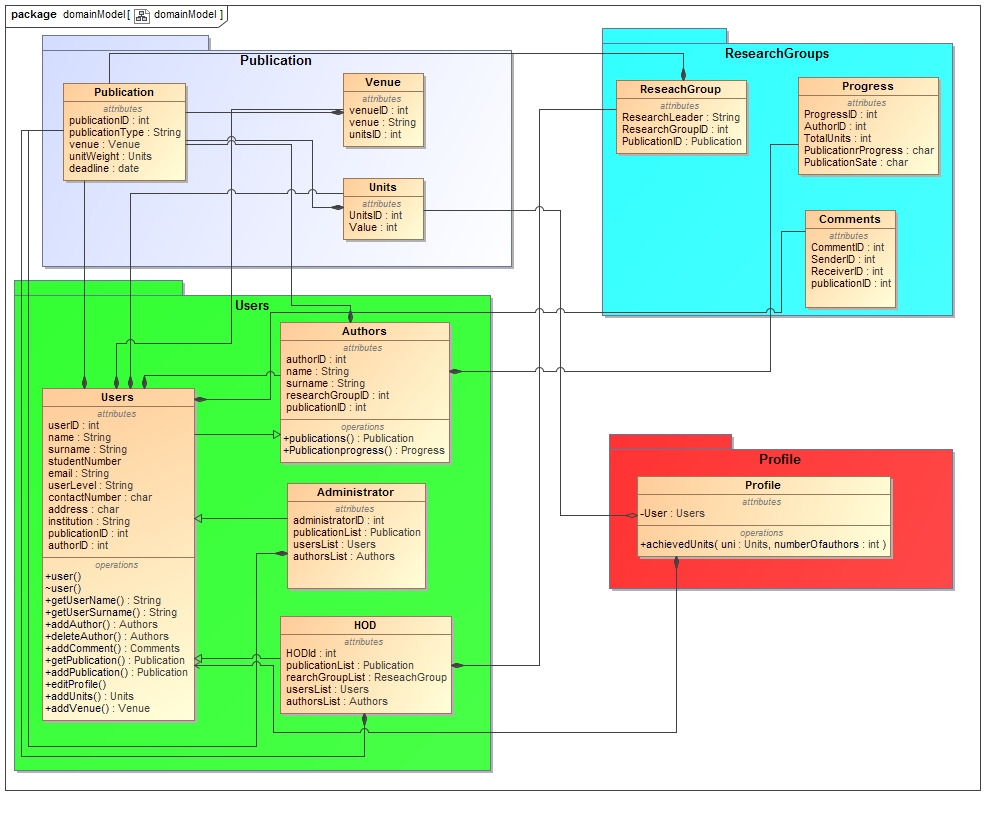
\includegraphics[width=130mm]{domainModel.jpg}
\caption{The domain model \label{overflow}}
\end{figure}
%----------------------------------------------------------------------------------------
% To be done by: Jacques & Jason
%----------------------------------------------------------------------------------------
\section{Open Issues}

Discuss in this section
\begin{itemize}
\item any aspects of the requirements which still need to be specified,
\item around which clarification is still required, as well as
\item any discovered inconsistencies in the requirements.
\end{itemize}


\end{document}
